\section{结果与讨论}
\subsection{特定条件下的性能评估}
为了评价新风的加热性能,机组特定条件下的室内环境(新风量为 $\qty{700}{\m^3/\hour} $,回风量为$\qty{1400}{\m^3/\hour} $,设定送风温度为$\qty{24}{\degreeCelsius} $)为例进行分析。实验结果如图~\ref{F:6} 所示。如图~\ref{E:6}(a) 所示,送风温度设定在$\qty{24}{\degreeCelsius} $附近波动,即最小送风量。空气温度为$\qty{22.7}{\degreeCelsius} $时,最高送风温度为$\qty{24.8}{\degreeCelsius} $,测试期间平均送风温度周期为$\qty{23.7}{\degreeCelsius} $,基本满足设定要求。这室内回风温度比较稳定,可以看到引入加热的新鲜空气不会额外增加室内热负荷。如图~\ref{E:6}(b) 所示,由于缺乏加湿设备,平均相对东风湿度仅为 7.4\%,平度相对回风湿度仅为 10.3\%。研究表面,低室内相对湿度使人感到明显的不适,降低工作效率,甚至影响人体健康。有必要增加室内相对湿度。常用的加湿方法主要有超声波加湿、干蒸汽加湿、离心加湿和湿介质加湿。此外,Ye 等人提出了一种小型化加湿模块,其组成平行多孔板的制作,并将其应用于室内风机盘管用于实验。实验结果表明,室内平均相对湿度较上年增加 33.8\% 比起非加湿条件。即使 $\qty{30}{\m^3/\hour} $的新鲜空气连续引入房间,该装置可以保持相对湿度为 30\%。

根据标准,要求的湿度比为 1 级热舒适度的数值为 $\qty{4.91}{\g/\kg}(\qty{22}{\degreeCelsius}, 30\%)$,送风湿度仅为$\qty{1.33}{\g/\kg}$
$(\qty{23.7}{\degreeCelsius}, 7.4\%)$。为达到 1 级热工要求的湿度比,在除人体的湿度散发外,就是还需要给房间补充水分,可以由加湿模块提供。该人工模块提供的湿度模块可计算为$\qty{4997}{\kg/\hour} $根据式~\ref{E:5}
\begin{equation}\label{E:5}
	H = \rho_s G_s (d_r - d_s) - nm_w
\end{equation}
式中,$H$为加湿模块提供的加湿嗯能力,$q_s, G_s, d_s$分别为密度、风量和湿度送风比。$d_r$为 1 级所需湿度比,$n$是人数,$m_w$是没人的耗湿量$\qty{75}{\g/\hour} $。

本实验中,为了考虑系统的简单性,没有加湿模块。由于供气量大,实际应用中可适当增加多孔板数量,加湿模块可放置在室内机加热盘管后面,增加送风的相对湿度。而且室外盘管结霜的问题依然存在在,严寒地区的热泵系统中。之前的学习表明,在室外温度$\qty{26.5}{\degreeCelsius} - \qty{1.0}{\degreeCelsius}{} $范围内会形成霜,并且霜在以下情况下会有所不同:应用于不同领域。目前应用最广泛的实际应用中的除霜方法是逆循环除霜。本文采用的机组为逆循环除霜,并可通过压缩机变频调节来适应负荷变化。本文主要分析新风、回风新风机组的制热性能(室内机)混合,室外机的结霜和除霜问题不予研究。

制冷剂参数是制冷剂的重要参数,保证实验系统安全稳定运行。如图~\ref{F:7} 展示特定条件下制冷剂参数随时间的变化状况。从图~\ref{F:7}(a) 可以看出,当室外温度基本恒定,变化趋势,压缩机吸气、排气和喷射温度相对平缓,波动均在$\qty{3}{\degreeCelsius} $以内。平均排气温度$\qty{56.8}{\degreeCelsius} $,平均喷射温度$\qty{14.7}{\degreeCelsius} $,平均吸气温度为$\qty{9.6}{\degreeCelsius} $。
从图~\ref{F:7}(b) 可以看出,压缩机的吸气、排气和喷射均未发生变化也很大。平均吸气压力为$\qty{0.52}{\MPa} $,平均排出压力$\qty{2.03}{\MPa} $,平均注入量压力为$\qty{0.68}{\MPa} $,平均压缩比为3.9,可以保证机组长期稳定运行。

实验过程中检测到的室外温度范围为$\qty{-21}{\degreeCelsius} - \qty{5}{\degreeCelsius}  $。虽然最低温度并没有降低。达不到空调室外计算湿度,基本可以覆盖哈尔滨冬季的大部分气温条件。为了验证机组在室外不同温度下,特别是$\qty{0}{\degreeCelsius} $以下的稳定性。在本部分中,检测的最低温度选择$\qty{-21}{\degreeCelsius} $,$\qty{5}{\degreeCelsius} $的区间,四种室外温度$\qty{-16}{\degreeCelsius} $、$\qty{-11}{\degreeCelsius} $、$\qty{-6}{\degreeCelsius} $被选作分析。实验过程中,新风量和回风量保持不变。有可能由图~\ref{F:8} 可见,随着室外温度的升高,平均吸气压力和吸气温度升高,平均排气压力和排气温度下降,且平均压缩比下降。当户外温度为$\qty{1}{\degreeCelsius} $时,平均压缩比仅为3.3.从图~\ref{F:8}(a) 还可以看出,平均温度混合空气的温度高于吸气温度,产生适合装置运行的冷凝压力。

\begin{table}[ht]
	\centering
	\caption{仪器的测量精度}
	\begin{tabular}{@{}lll@{}}
		\toprule
		测试仪器 & 测量范围 & 误差 \\ \midrule
		T---型热电偶 & $-50-\qty{140}{\degreeCelsius}$ & $\pm \qty{0.1}{\degreeCelsius} $ \\ 
		压力传感器 & 吸力: $0-\qty{1.6}{\MPa} $ & $\pm 0.5$FS \\
			& 注射: $0-\qty{3}{\MPa} $ & $\pm 0.5$FS \\
			& 其他三种: $0-\qty{5}{\MPa} $ & $\pm 0.5$FS \\
		温湿度传感器 & T: $-40-\qty{140}{\degreeCelsius} $ & T: $\pm \qty{0.2}{\degreeCelsius} $ \\
					 & RH: 0-100\% & RH: $\pm 2\%$ \\ 
		功率计	& 室外: $0-\qty{6600}{\W} $ & $\pm 0.5\%$FS \\
				& 室内: $0-\qty{1100}{\W} $ & $\pm 0.5\%$FS \\
		热线风速仪 & $0-\qty{40}{\m/\s}$ & $\pm$($3\% + \qty{0.03}{\m/\s}$) \\ \bottomrule
	\end{tabular}
	\label{T:2}
\end{table}

\begin{figure}[htbp]
	\centering
	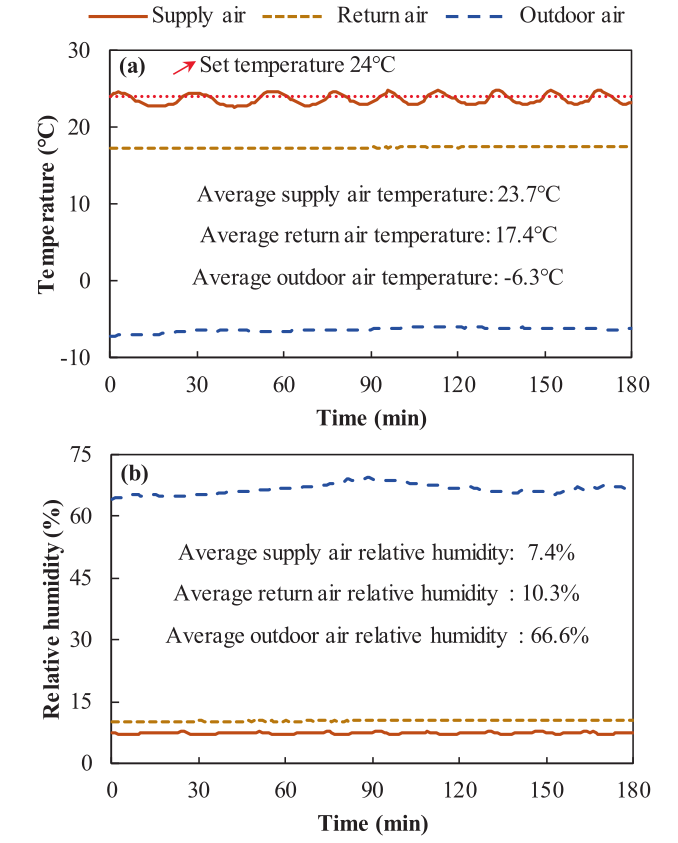
\includegraphics[width=0.7\textwidth]{figure/figure_6}
	\caption{室内外环境参数(室外温度: $\qty{-6}{\degreeCelsius}\pm \qty{0.5}{\degreeCelsius}  $)}
	\label{F:6}
\end{figure}

\begin{figure}[htbp]
	\centering
	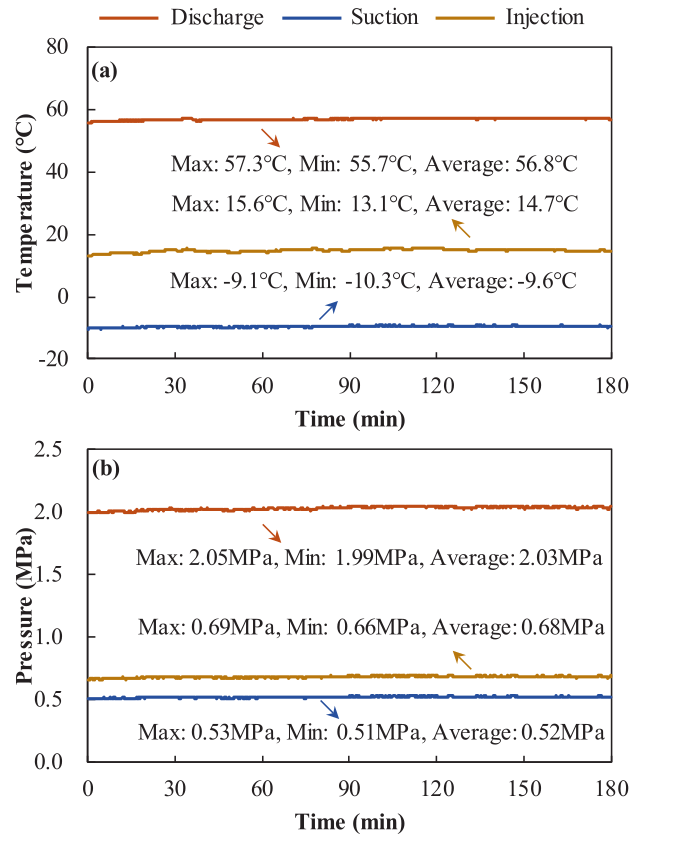
\includegraphics[width=0.7\textwidth]{figure/figure_7}
	\caption{制冷剂参数随时间的变化(室外温度: $\qty{-6}{\degreeCelsius}\pm \qty{0.5}{\degreeCelsius}  $)}
	\label{F:7}
\end{figure}

\begin{figure}
	\centering
	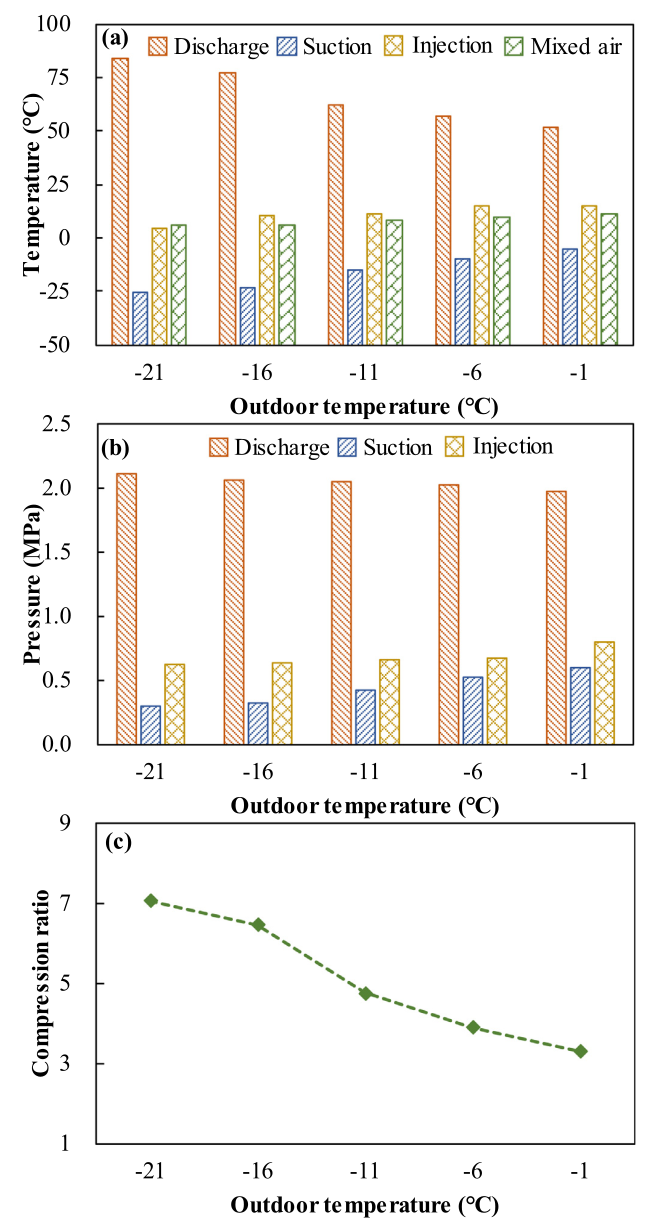
\includegraphics[width=0.7\textwidth]{figure/figure_8}
	\caption{制冷参数随室外温度的变化}
	\label{F:8}
\end{figure}

由于吸气压力是影响注射压力的主要因素,因此注射压力的变化趋势与吸气压力相同。喷射温度等于喷射制冷剂的饱和温度与喷射制冷剂的过热度之和。由于喷射制冷剂的饱和温度是由喷射压力决定的,因此喷射温度和喷射压力具有相同的变化趋势。

如图~\ref{F:9} 所示,每小时的制热量和每小时的耗电量随室外温度的变化而变化。从图~\ref{F:9} 可以看出,随着室外温度的降低,新风机组的制热量和压缩机的功耗增加。这是因为室外温度越低,新风的热负荷越大,导致机组的制热量增加。图~\ref{F:10} 图~\ref{F:11} 显示了每小时 COP 随室外温度的变化。随着室外温度的降低,喷射压力降低(图~\ref{F:8}(b),压缩比增大(图~\ref{F:8}(c)),每小时COP降低并基本呈线性变化(图~\ref{F:10})。当室外温度为$\qty{4.9}{\degreeCelsius} $时,热泵 COP 为 4.29,即使室外温度降至$\qty{20.9}{\degreeCelsius} $,热泵 COP 仍可达到2.46。

\begin{figure}
	\centering
	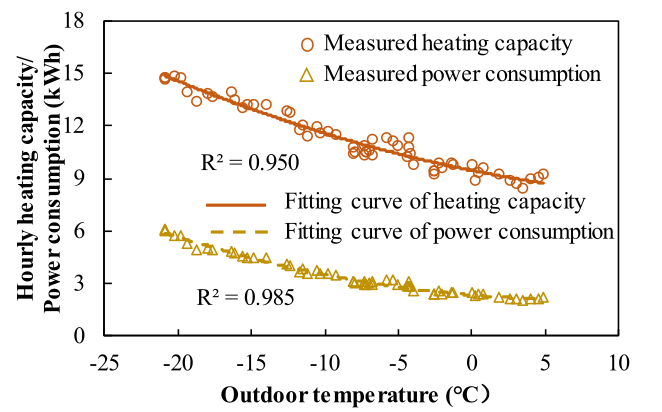
\includegraphics[width=0.7\textwidth]{figure/figure_9}
	\caption{每小时制热量和耗电量随室外温度的变化}
	\label{F:9}
\end{figure}

\begin{figure}
	\centering
	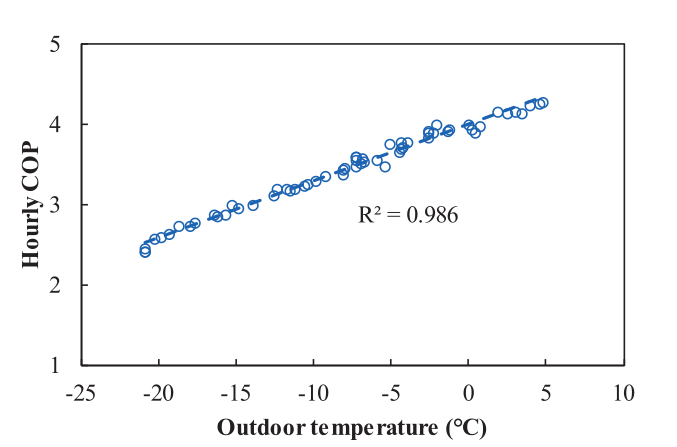
\includegraphics[width=0.7\textwidth]{figure/figure_10}
	\caption{每小时 COP 随室外温度的变化}
	\label{F:10}
\end{figure}

为了验证新风与回风混合的空气源热泵新风机组的节能效果,将严寒地区常用的两台热回收新风机组进行了对比。两台热回收新风机组示意图如图~\ref{F:11} 所示。考虑到热回收装置内结霜等问题,室外空气一般先用电预热至$\qty{5}{\degreeCelsius} $后送至板式热回收器设备。案例 3 为案例 2 经过热回收装置后的空气通过空气源热泵 (ASHP)。室内机加热至送风温度$\qty{24}{\degreeCelsius} $。图~\ref{F:11}(a)),而案例3为制热通过电加热器调节送风温度(图~\ref{F:11}(b))。计算过程中,工况 2 和 3 的新风量和设定温度与工况 1 相同,回风量取新风量的 90\%。

通过电预热至$\qty{5}{\degreeCelsius} $的室外新风制热能力$Q_1$和耗电量$W_1$(电热效率为 1),可由式~\ref{E:6} 计算
\begin{equation}\label{E:6}
	Q_1 = W_1 = \frac{G_W \rho_W C_W (t_P - t_W)}{3600} 
\end{equation}
其中,下标$W, P$分别代表图~\ref{F:11} 中的 W 点和 P 点。

板式热回收装置的热回收效率$\nu$按式~\ref{E:7} 计算,制热量 $Q_2$由式~\ref{E:8} 计算。这部分没有能量消耗,$W_2 = 0$。在式~\ref{E:8} 中, $\nu$为显热回收效率,本次计算取 70\%。
\begin{equation}\label{E:7}
	\nu = \frac{G_S (t_P - t_J)}{G_{min} (t_P - t_N)} 
\end{equation}
\begin{equation}\label{E:8}
	Q_2 = \frac{G_P \rho_P (t_J - t_P)}{3600} 
\end{equation}
式中,$G_{min}$是送风量和回风量的最小值,小标 S、J、N 分别代表图~\ref{F:11} 的 S、J、N 点。

新鲜空气经过热回收装置后,通过电加热($Q_3$)或空气源热泵室内机($Q'_3$)加热至$\qty{24}{\degreeCelsius} $。热量 $Q_3 = Q'_3 $可从式~\ref{9}中计算。点热能消耗$W_3$与$Q_3$相同,空气源热泵室外机的能耗$W'_3$可按式~\ref{E:10} 来计算。
\begin{equation}\label{E:9}
	Q_3 = Q'_3 = W_3 = \frac{G_j \rho_J c_j(t_S - t_J)}{3600} 
\end{equation}
\begin{equation}\label{E:10}
	W'_3 = \frac{Q'_3}{COP} 
\end{equation}

案例 2 中,进入室内机的空气温度为$\qty{13.2}{\degreeCelsius} $,而案例 1 中,进入室内机的空气温度(混合空气温度,图~\ref{E:8}(a))。随着室外温度的变化而变化,但温差为低于$\qty{8}{\degreeCelsius} $。为了方便比较,式中的 COP 取式~\ref{E:10} 作为案例 1 的 COP 和 新风单元对应的环境温度。

热回收新风组能量计算结果如表~\ref{T:3}。

情况 2 和 3 下的新风 COP 可由式~\ref{E:11} 和 \ref{E:12}

\begin{equation}\label{E:11}
	COP' = \frac{Q_1 + Q_2 + Q_3}{W_1 + W'_3} 
\end{equation}

\begin{equation}\label{E:12}
	COP^{''} = \frac{Q_1 + Q_2 + Q_3}{W_1 + W_3} 
\end{equation}

图~\ref{F:12} 显示了三种不同类型新风机组的 COP。从图~\ref{F:12} 可以看出,当采用电加热进行新风预热时,案例 2 和案例 3 的COP值较低。但由于案例 2 采用空气源热泵对热回收后的空气进行加热, 其COP 值大于案例 3 采用的电加热方式。相比之下,案例 1 的 COP 高于案例 3。案例 2 和案例 3 在不同的室外温度下。当室外温度为$\qty{29}{\degreeCelsius} $时,案例 1 的 COP 可以达到2.46,而案例 2 的COP仅为1.44,案例 3 的COP 更低,只有1.21。可见,本文选用的新风机组节能效果显着。另外,本次实验中,为了系统的简单性,没有设置热回收装置。

\begin{figure}
	\centering
	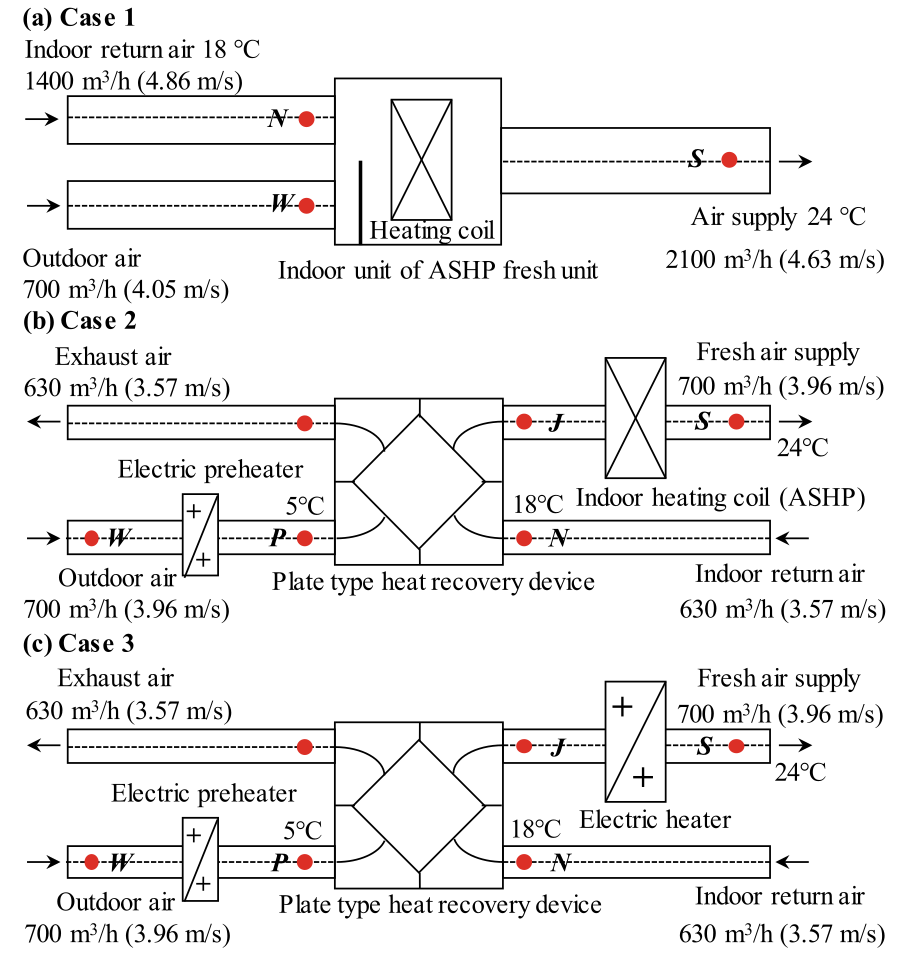
\includegraphics[width=\textwidth]{figure/figure_11}
	\caption{热回收新风机组示意图}
	\label{F:11}
\end{figure}

\begin{table}[ht]
\centering	
\caption{能量计算结果}
\begin{tabular}{@{}lllll@{}}
	\toprule
	室外温度 & $Q_1 = W_1$ & $Q_2$ & $Q_3=Q'_3=W_3$ & $W'_3$ \\ \midrule
	$\qty{20.9}{\degreeCelsius} $ & $\qty{7.10}{\kW} $ & $\qty{2.04}{\kW} $ & $\qty{2.60}{\kW} $ & $\qty{1.06}{\kW} $ \\
	$\qty{16.1}{\degreeCelsius} $ & $\qty{5.80}{\kW} $ & $\qty{2.04}{\kW} $ & $\qty{2.60}{\kW} $ & $\qty{0.91}{\kW} $ \\
	$\qty{11.2}{\degreeCelsius} $ & $\qty{4.45}{\kW} $ & $\qty{2.04}{\kW} $ & $\qty{2.60}{\kW} $ & $\qty{0.81}{\kW} $ \\
	$\qty{5.8}{\degreeCelsius} $ & $\qty{2.97}{\kW} $ & $\qty{2.04}{\kW} $ & $\qty{2.60}{\kW} $ & $\qty{0.73}{\kW} $ \\
	$\qty{1.2}{\degreeCelsius} $ & $\qty{1.70}{\kW} $ & $\qty{2.04}{\kW} $ & $\qty{2.60}{\kW} $ & $\qty{0.66}{\kW} $ \\ \bottomrule
\end{tabular}
\label{T:3}
\end{table}

\subsection{不同回风量下的性能评估}
回风阀全开时,风量略大于$\qty{1800}{\m^3/hour} $,最大风量设定为$\qty{1800}{\m^3/\hour}$。由图~\ref{F:4} 可知,具体工况下回风量为$\qty{1400}{\m^3/\hour} $,混合风温度为$\qty{3.0}{\degreeCelsius} $,可以避免换热器结霜。同时选择极端工况,即回风量为$\qty{400}{\m^3/\hour} $,验证低回风量的可能性。实验过程中,新风量保持在$\qty{700}{\m^3/]hour} $板式热回收装置的回收设定温度$\qty{24}{\degreeCelsius}$。图~\ref{F:13} 为回风量$\qty{400}{\m^3/\hour} $时制冷剂参数随时间的变化。从图~\ref{F:13}(a) 可以看出,吸气温度比较稳定,平均值$\qty{12.1}{\degreeCelsius} $,理论混合空气温度$\qty{2.7}{\degreeCelsius} $。排气温度和喷射温度波动压力较大,平均排出温度为$\qty{47.6}{\degreeCelsius} $,平均注射温度$\qty{8.8}{\degreeCelsius} $。从图~\ref{F:13}(b) 可以看出,排出压力波动较大,范围为$1.48 - \qty{2.55}{\MPa} $,平均排出压力为$\qty{1.72}{\MPa} $。注射压力波动缓慢,平均注射压力$\qty{0.76}{\MPa} $,吸入压力最稳定,平均值为$\qty{0.45}{\MPa} $。压缩机压缩比在 3.3 \textasciitilde 5.0 之间,平均压缩比 3.8 (图~\ref{F:13}(c)),机组运行稳定性较差。考虑的原因是回风量小,冷凝测压力低,节流装置液流不足。

\begin{figure}[htbp]
	\centering
	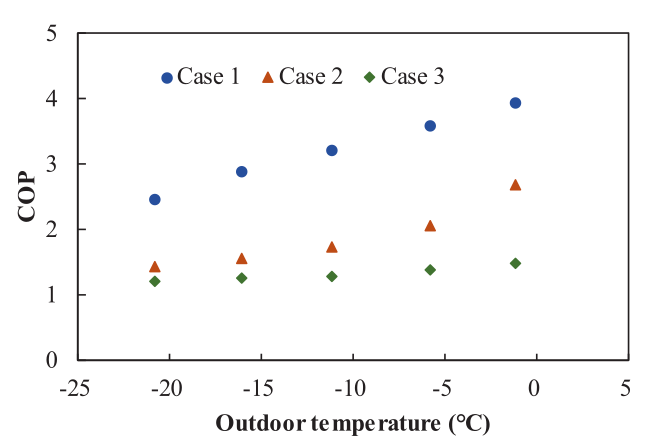
\includegraphics[width=0.7\textwidth]{figure/figure_12}
	\caption{不同类型新风机组的 COP}
	\label{F:12}
\end{figure}

\begin{figure}[htbp]
	\centering
	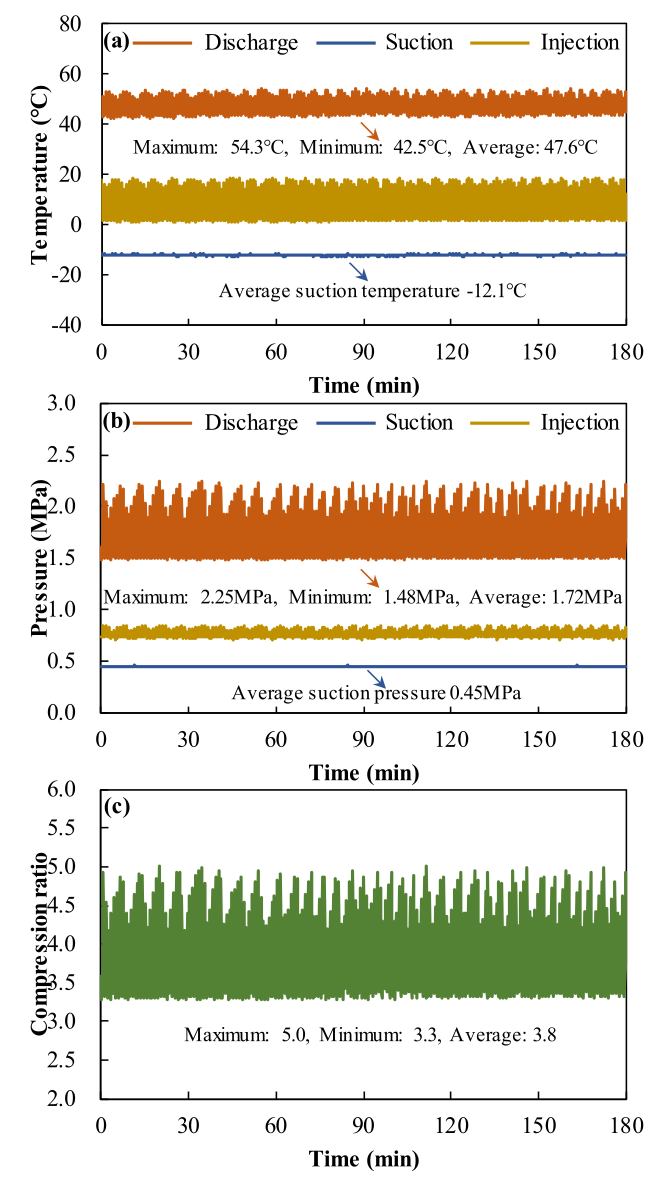
\includegraphics[width=0.7\textwidth]{figure/figure_13}
	\caption{制冷剂参数随时间的变化 (室外温度: $\qty{6}{\degreeCelsius} \pm \qty{0.5}{\degreeCelsius} $)}
	\label{F:13}
\end{figure}

图~\ref{F:14} 为回风量 $\qty{400}{\m^3/\hour} $时送风参数随时间的变化趋势。从图~\ref{F:14} 可以看出,最高送风温度达到$\qty{26.7}{\degreeCelsius} $,最低送风温度仅为$\qty{20.8}{\degreeCelsius} $。送风参数波动比较明显,无法持续稳定地输送新鲜空气进入房间。这进一步证实了机组的不稳定性。这进一步证实了回风量为$\qty{400}{\m^3/\hour} $ 时机组运行的不稳定性。当回风量为回风量为$\qty{1800}{\m^3/\hour} $时,机组运行状态和送风参数的变化趋势与回风量为 $\qty{400}{\m^3/\hour} $时相同。运行状态和送风参数的变化趋势与回风量为$\qty{1400}{\m^3/\hour} $ 时相同(图~\ref{F:6}和图~\ref{F:7}),在此不再赘述。

\begin{figure}[htbp]
	\centering
	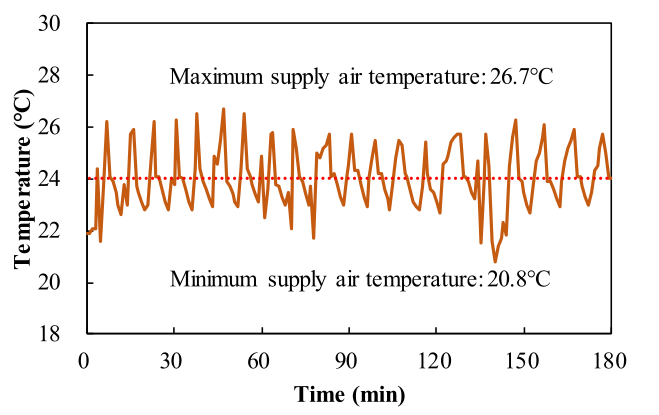
\includegraphics[width=0.7\textwidth]{figure/figure_14}
	\caption{送风参数随时间的变化 (室外温度: $\qty{6}{\degreeCelsius} \pm \qty{0.5}{\degreeCelsius} $)}
	\label{F:14}
\end{figure}
 
由于回风量较低时机组运行稳定性较差,因此 COP 计算不准确。本文仅比较了回风量为$\qty{1400}{\m^3/\hour} $ 和$\qty{1800}{\m^3/\hour} $两种情况下的热泵 COP,如图~\ref{F:15} 所示。从图~\ref{F:15} 中可以看出,当室外温度相同时,回风量越大,热泵的 COP 越高。相同时,回风量越大,热泵 COP 越高。测试期间,回风量为$\qty{1800}{\m^3/\hour} $ 的 COP 比回风量为$\qty{1400}{\m^3/\hour} $ 的 COP 高出 3.5\%-9.0\%。

\begin{figure}[htbp]
	\centering
	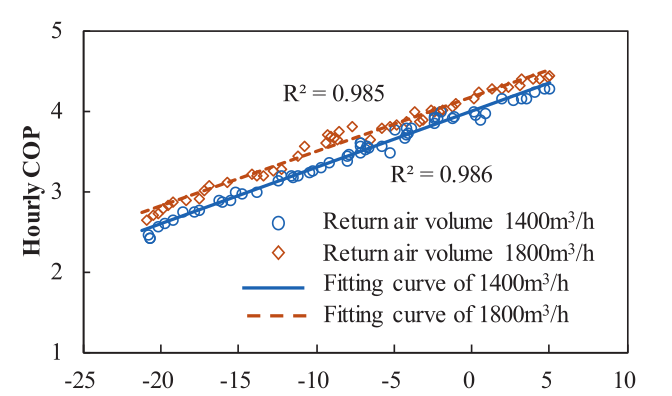
\includegraphics[width=0.7\textwidth]{figure/figure_15}
	\caption{不同回风量下热泵 COP 对比}
	\label{F:15}
\end{figure}

新风装置加热循环的理论压力-焓图如图~\ref{F:16} 所示。如图~\ref{F:16} 所示。制冷剂流量可由公式~\ref{E:13}
\begin{equation}\label{E:13}
	m = \frac{Q}{h_3 - h_4} 
\end{equation}
$m$是制冷剂流量,$h_3, h_4$是点 3、4 处的值。

\begin{figure}[htbp]
	\centering
	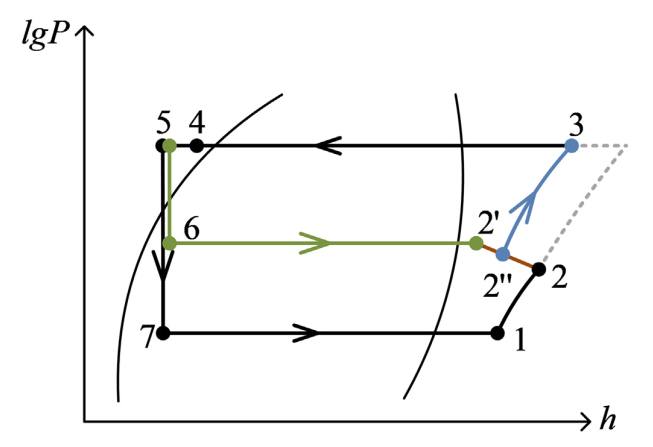
\includegraphics[width=0.7\textwidth]{figure/figure_16}
	\caption{加热循环的理论压力--焓图}
	\label{F:16}
\end{figure}

取室外温度$\qty{-6}{\degreeCelsius} $进行分析,如表~\ref{T:4} 所示。表~\ref{T:4} 不同回风量下机组运行参数比较不同回风量下的机组运行参数对比。从表~\ref{T:4} 可以看出在回风量为$\qty{1400}{\m^3/\hour} $  和$\qty{1800}{\m^3/\hour} $  的稳定条件下,回风量的增加,风机的吸入压力和排出压力也随之增加。压缩机的吸气压力和排气压力都增加了,导致蒸发温度增加$\qty{3.12}{\degreeCelsius} $,冷凝温度增加$\qty{1.54}{\degreeCelsius} $。由于蒸发温度对 COP 的影响大于冷凝温度,因此$\qty{1400}{\m^3/\hour} $ 回风量的 COP 大于$\qty{1400}{\m^3/\hour} $ 回风量的 COP。。从制冷剂流量也可以看出,随着回风量的增加,制冷剂流量增加,机组的制热能力增加,油压功耗降低,因此热泵的 COP 增加。

\begin{table}[ht]
	\centering
	\caption{同回风量下机组运行参数对比}
	\begin{tabular}{@{}llllll@{}}
		\toprule
		回风量($\unit{\m^3/\hour}) $ & 吸入压力($\unit{\MPa}) $ & 蒸发温度($\unit{\degreeCelsius} $) & 排气压力($\unit{\MPa}) $ & 冷凝温度($\unit{\degreeCelsius}) $ & 制冷剂流量($\unit{\kg/\s} $) \\ \midrule
		400 & 0.45 & 16.87 & 1.48-2.25 & 20.81-36.93 & 0.0421-0.0483 \\
		1400 & 0.52 & 12.85 & 2.03 & 32.81 & 0.0489 \\
		1800 & 0.58 & 9.73 & 2.11 & 35.35 & 0.0517 \\ \bottomrule
	\end{tabular}
	\label{T:4}
\end{table}

\subsection{不同设定温度下的性能评估}
为了评估机组在不同设定温度下的性能,
本$\qty{20}{\degreeCelsius} $,$\qty{22}{\degreeCelsius} $,$\qty{24}{\degreeCelsius} $,$\qty{26}{\degreeCelsius}$,$\qty{28}{\degreeCelsius} $部分选取了五个条件进行测试。试验时新风量为$\qty{700}{\m^3/\hour} $,回风量为$\qty{700}{\m^3/\hour} $,室外温度保持在$\qty{6}{\degreeCelsius} \pm \qty{0.5}{\degreeCelsius} $。图~\ref{F:17} 为平均送风温度和每小时的情况。机组在不同设定温度下连续稳定运行的制热量。从图~\ref{F:17} 可以看出,当设定温度为$\qty{26}{\degreeCelsius} $及以下时,送风温度基本能满足设定温度值,且机组的制热量随着设定温度的升高而增加,几乎与线性。但当设定温度为$\qty{28}{\degreeCelsius} $时,送风温度明显低于$\qty{28}{\degreeCelsius} $。考虑的原因可能是设定温度太大,机组的制热量无法满足设定的要求温度。

\begin{figure}[htbp]
	\centering
	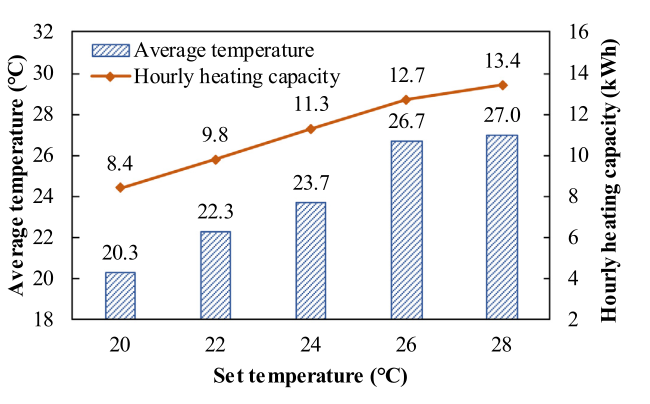
\includegraphics[width=0.7\textwidth]{figure/figure_17}
	\caption{不同设定温度下的平均送风温度和每小时制热量}
	\label{F:17}
\end{figure}

图~\ref{F:18} 为不同设定温度下热泵COP的比较。从图~\ref{F:18} 可以看出,随着设定温度的升高,COP 呈现先增大后减小的趋势,在设定温度为$\qty{24}{\degreeCelsius} $时达到最大值。设定温度低,机组低频运行效率低。随着设定温度的升高,当机组运行频率增加到一定值时,机组制热量增大,换热器面积相对不足,系统运行工况恶化,COP值下降。另外,如果设定温度升高,冷凝侧温(1)通过新风与回风混合提高冷凝压力,使空气源热泵新风机组在严寒地区稳定运行,冷凝测温度太大,也会导致COP下降。

\begin{figure}[htbp]
	\centering
	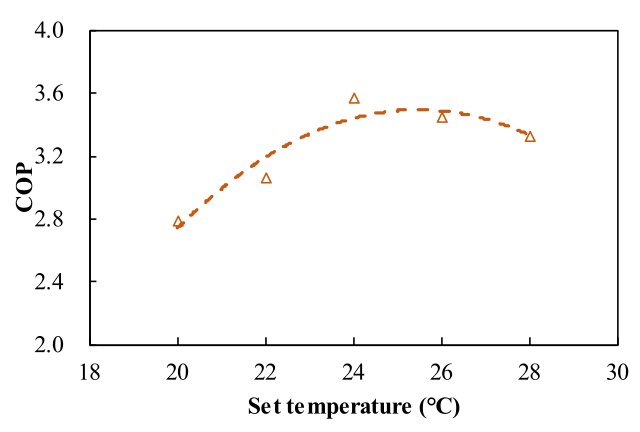
\includegraphics[width=0.7\textwidth]{figure/figure_18}
	\caption{不同设定温度下的热泵 COP}
	\label{F:18}
\end{figure}
